\section{Introduction}
\label{sec:intro}

\subsection{Motivation}
The trajectory around a track that allows a given vehicle to traverse the circuit in the minimum amount of time is called the ideal racing line. There are a lot of parameters that determine the minimum lap time. In general it is a trade-off between the length of the taken line and the speed carried around the track, which in most cases turns out to be the line with the least curvature.  
Needless to say, in a race this is the path every driver wants to take. In reality, however, this isn't an easy task. In order to achieve best times, a racing driver has to remember exactly which corner of the track comes next, how fast they can take this corner, see how the car is positioned on the track and process much more information.
To assist aspiring drivers feel like professionals, we implemented a racing driver analysis system, that is capable of recording, comparing and evaluating race related data. The system saves a complete history of the many sensor data values, like speed, throttle position and safety relevant features, like engine temperature, the car produces and tracks the car on the course using a combination of different methods.
This car tracking will be the main focus of this thesis. The comparison of two drivers requires very robust measurements, that return the same result for every given input.
The most common tracking method, GPS, relies on external sources, namely satellites that communicate with the GPS device. The biggest problem with this traditional approach is, that GPS isn't fully available everywhere. Especially on remote areas, which is where most race tracks are, there tends to not be complete coverage. This would result in faulty results and incomparable racing lines.
In order to break away from these dependencies, we used a camera-based approach. This allows us to track the relative translation and rotation of the vehicle independent of its speed, location or surroundings.
Apart from the recording of these racing lines, this paper also discusses how to process the obtained data so that they provide a useful support for racing drivers.

\subsection{Project Scope}
During the one year long bachelor project "Feel the Car - Automatic A\-no\-ma\-ly Detection for Unstructured Test Drive Data" at the Hasso-Plattner-Institute, Potsdam, I worked together with four fellow students and in cooperation with Mercedes-AMG on analyzing video and sensor data from car test drives.
Part of the project was to find a possibility to retrospectively evaluate a race for a given driver. This is especially useful for AMGs Driving Academy \footnote{\url{http://www.mercedes-amg.com/driving-academy/}}, which is a service that lets non-professional drivers drive on race tracks and become a racing driver. To achieve this goal, and other requirements, such as detecting potholes on the street or security relevant warning signs in races, we used a stereo camera and a mini-computer, that processed the incoming raw data.
Additionally, an On-Board-Diagnostic 2 (OBD-II) dongle was used to extract the sensor data that cars have already integrated.
The analyzed result was then displayed in our web application which also provided a driver overview so every driver had a detailed overview over their recorded laps.
\clearpage

\subsection{Problem Introduction/Description/Context}

\begin{figure}[!ht]
	\centering
	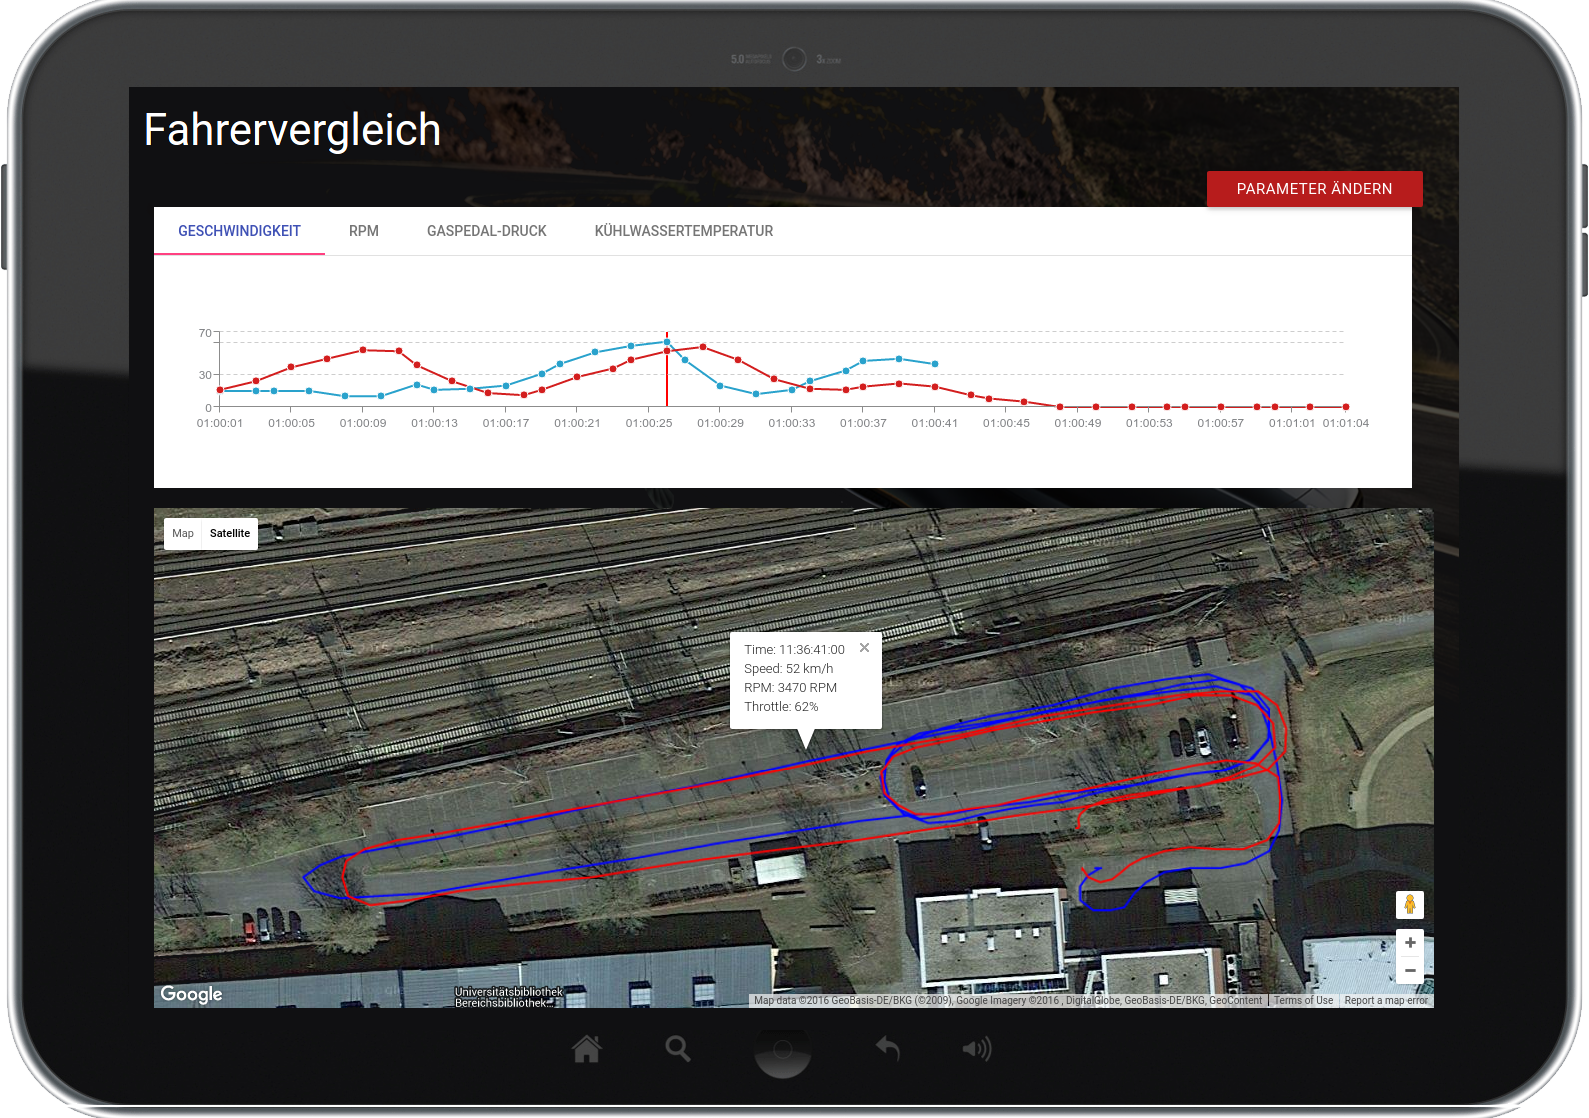
\includegraphics[width=\textwidth]{tablet_with_driver_comparison}
	\caption{Driver Comparison}
	\label{fig:comparison_with_overlay}
\end{figure}

Initially, our task was to analyze existing video material from test drives made by AMG. The exact specifications of this analysis were specified at a meeting with AMG and developed to mainly consist of video- and sensor-based driving aids for drivers at the AMG Driving Academy. Besides the detection of security-relevant events, like warning flags, cars leaving the track into the gravel bed or potholes on the street, we also wanted to find a way to compare and evaluate the driving behavior of two drivers.
During our first tests, which started with a mobile phone camera, we found out, that there are a lot of challenges and prerequisites in video analysis. For example, every camera has to be calibrated first, to compute for the individual distortion a camera lens causes. This is not only a fairly complex and accurate task, it also prevents an easy replacement of camera hardware.\\
This made us look into alternatives and we decided to use a stereo camera. A stereo (or 3D) camera is able to determine metric measurements from the camera image, which enables it to calibrate itself. Also the additional information we can extract from a 3D image made a more accurate and faster detection possible.\\

\begin{figure}[!ht]
	\begin{minipage}[b]{.45\textwidth}
		\centering
		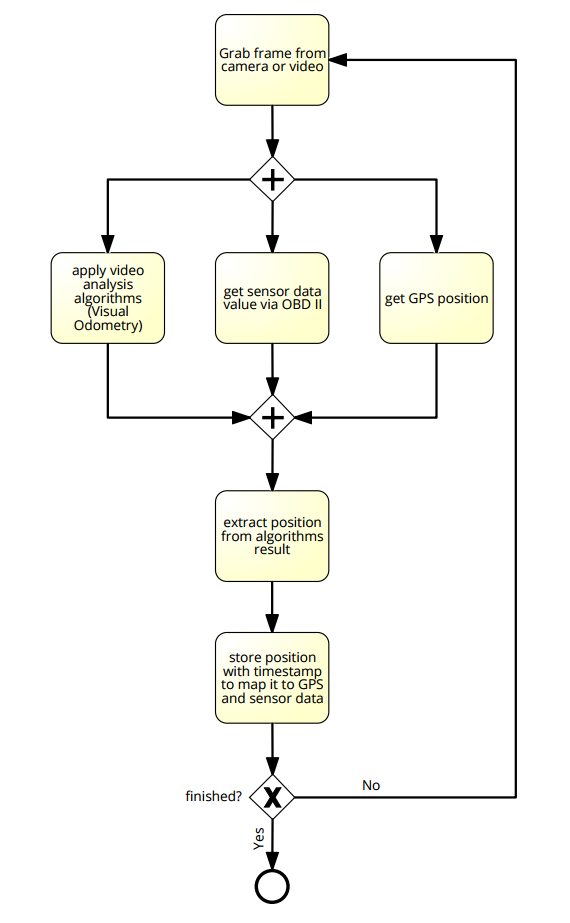
\includegraphics[height=8cm]{racing_line_recording}
		\caption{Process Diagram Racing Line Recording}
		\label{fig:racing_line_recording}
	\end{minipage}
	\hfill
	\begin{minipage}[b]{.45\textwidth}
		\centering
		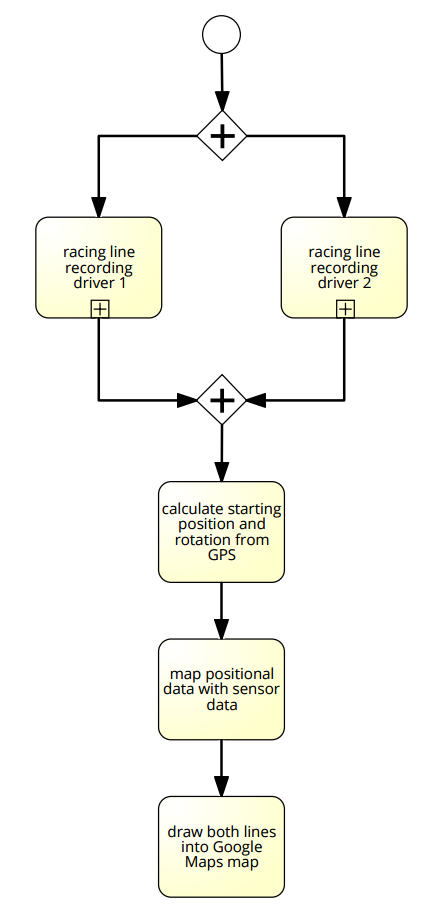
\includegraphics[height=8cm]{racing_line_comparison}
		\caption{Process Diagram Racing Line Comparison}
		\label{fig:racing_line_comparison}
	\end{minipage}
\end{figure}

Using techniques that will be described in section \ref{sec:algorithm}, we were able to record the racing line of a car based on a stereo video and GPS. Together with the extracted sensor data from the OBD II interface, we stored the points in a database. The process can be seen in diagram \ref{fig:racing_line_recording}.

Diagram \ref{fig:racing_line_comparison} shows how the recorded racing lines can then be compared. We decided to use a Google Maps integration to properly determine where on the track potential improvements can be found. Interesting data values were displayed by coloring in the racing line, in case of the detailed driver view (figure \ref{fig:driver_detail}) or using an info window, which gives an overview of the data at a given point (figure \ref{fig:comparison_with_overlay}).

\begin{figure}[!ht]
	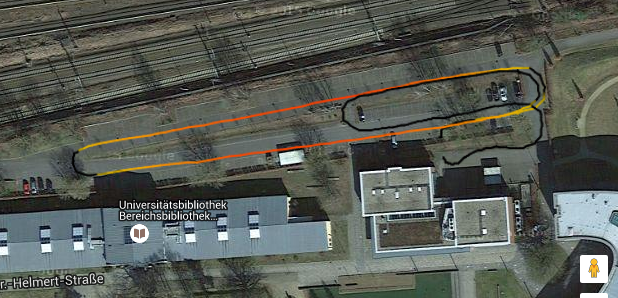
\includegraphics[width=\textwidth]{driver_detail_screenshot}
	\caption{Detailed Driver Overview}
	\label{fig:driver_detail}
\end{figure}

\clearpage